\subsection{Data view}

There are two perspectives on data in the system: One is the interaction with the MySQL remote database
and the other is the interaction with the local file system used in \emph{LocalFileModel}.

\subsubsection{Remote database view}
The mapping between the database and the logical classes is found in \\\emph{MySQLModel.edmx} in the
\SOP{} project.

Most of the mapping is as straight forward as it gets: Properties map to fields of the corresponding value.
However, in the relationship of the entities there are some important details.

The first point that is important to make is that users are defined in the data as tuples of emails
and passwords and that between users and projects there is a many-to-many relation. This manifests
in the ProjectUser table, holding references to both. In effect this means that several users may 
have access to the same projects, and that one owner may have access to several projects.

\begin{figure}[htb]
	\centering
	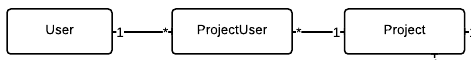
\includegraphics[width=0.75\textwidth]{Software_architecture/graphics/db-user-project.png}
	\caption{The many-to-many relationship between users and project.}
	\label{fig:db-user-project}
\end{figure}

\begin{figure}[htb]
	\centering
	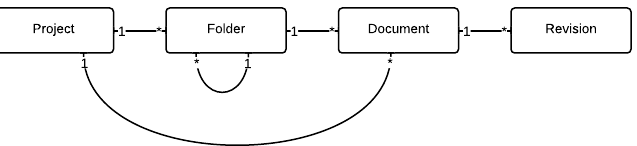
\includegraphics[width=1.0\textwidth]{Software_architecture/graphics/db-project-folder-document.png}
	\caption{The one-to-many relationships between projects, folders, documents and revisions.}
	\label{fig:db-project-folder-document}
\end{figure}

The Folder table contains a reference to a Folder OR a reference to a Project. This is important as
it may live in either of these. It should never have both, but this is not a constraint inherent to
the database. This manifests in a one-to-many relationship, where a parent project or folder may have
many child folders.

Documents have the same references as Folders, and results in the same kind of relationship.

Revisions have references to Documents, resulting in a one-to-many relationship where a single document
may have several revisions tied to it.

\subsubsection{File system view}
The logical classes used in the system (see Section \ref{sec:logicalview}) map almost precisely to a
traditional file system hierarchy. In the file system they are represented as follows: Projects are
represented as folders, found in the root of the data folder (in \emph{<userdir>/AppData/Roaming/SliceOfPie});
Folders are folders inside the projects; Documents are files with a \emph{.txt} ending, inside either folders
or projects.